\section{Microarchitecture-Level Protection}

This section discusses hardware protection mechanisms that are necessary
to implement timing compartments on typical multi-core processors.

At a glance, designing a full processor with timing channel
protection may seem rather straightforward because there exist previous 
studies on major components such as 
shared caches \cite{percival}, 
on-chip interconnect \cite{yaonocs, surfnoc}, and the memory controller \cite{ushpca14}.
However, through the design process, we found three new sources of timing 
channels in module interfaces that were not identified previously, found a
bug in the memory controller protection \cite{ushpca14}, and found that cache 
coherence protocols can cause interference even among programs that do not 
share data with each other.
We also found that time multiplexing schemes
must be carefully coordinated in order to avoid 
unnecessarily high overheads. 

%<<<<<<< HEAD
%=======
%\subsection{Baseline Architecture}
%
%    \begin{figure}
%        \begin{center}
%            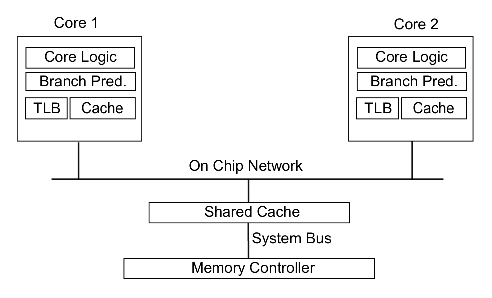
\includegraphics{figs/baseline.eps}
%            \caption{Baseline multi-core architecture.}
%            \label{fig:baseline}
%        \end{center}
%    \end{figure}
%
%Figure \ref{fig:baseline} shows a baseline multi-core architecture that we
%extend with timing compartments in this paper. The architecture
%has multiple cores, each with a core pipeline, a branch predictor, a TLB,
%and one or more private caches.  The cores are connected to a shared cache via 
%an on chip network. A shared system bus connects the shared cache to a memory 
%controller that manages requests to main memory.
%We assume that each core may be time shared by multiple timing
%compartments, but only one timing compartment, which we say is active, may run 
%on each core
%at a time. This assumption can be relaxed if timing channel protection
%is added to per-core resources.
%
%\Ed{Perhaps move all the assumption that we make here?}
%
%>>>>>>> e53c686ccc6b2272048753993b59beaee62211b0
%A trusted software layer (such as an operating system) allocates software 
%entities (such as processes) to the cores. 

\subsection{General Protection Approaches}
\label{sec:general_approaches}

Here, we present a classification of microarchitectural timing 
channels and a framework of general solutions to address each type.
Because we aim to prevent both side-channel and cover-channel attacks,
the approach is designed to remove interference rather than mitigating it.
%We follow these approaches to design our
%protection mechanisms. These approaches also provide guidelines to
%develop new protection mechanisms for components that are not included in
%our baseline architecture.

\subsubsection{TCID}

The hardware protection mechanisms need to track which timing compartment (TC)
each request belongs to and handle the requests accordingly. 
For this purpose, each core has a register that 
stores the timing compartment ID (TCID) of the TC currently active on that 
core. This is used to derive the tags that are appended to requests originating 
from that core. The TCID is $log\ n$ bits where $n$ is the number of cores in 
the processor.
Events such as network packets or cache accesses that use shared resources are 
tagged with the TCID of the corresponding core.  The timing channel protection 
mechanisms use this TCID to distinguish accesses
from among different timing compartments.

\subsubsection{Sources of Inter-Program Timing Channels}

There exists an inter-progam timing channel from one entity (say $E1$)
to another ($E2$) when the timing of an event in $E1$ can be affected by 
the behavior of $E2$.

There are two types of inter-program timing channels in hardware: state-based
and contention-based.
A \emph{state-based} timing channel occurs when there is a state element 
that is shared among multiple entities and whose
content affects timing of an event.
For example, a conventional shared cache has state-based timing channels, 
because cache hits are faster than misses.
A \emph{contention-based} timing channel occurs when multiple entities 
share a resource that can only handle a finite number of requests at a time.
Conventional buses have contention-based timing channels.

\subsubsection{State-Based Timing Channel Protection}

%Caches, TLBs, and branch predictors all have state-based timing channels.  In 
%each, requests that use an entry that is present in the state elements (e.g.  
%cache hits) are faster than requests to entries not present (e.g. cache 
%misses). The state elements can contain a finite number of entries, so entries 
%must be evicted and replaced with new ones. One software entity can evict 
%entries owned by another, causing interference and timing channel leakage if 
%the choice of entries evicted correlates with a secret. 
In general, state-based timing channels can be removed by applying 
flattening, partitioning, or flushing.
Flattening eliminates the dependence of access time on the state by forcing 
every access to finish in the same (worst case) time. For example, to remove 
timing interference in the row buffers of DRAM, all DRAM accesses may be 
treated as a row buffer miss.
%For some components, this is a brute-force approach. 
Applied to caches, every 
access must be treated as a miss, so this is equivalent to removing the cache. 

Partitioning removes interference by ensuring that each entity can
only affect a disjoint subset of state elements. The partitions
should not change dynamically depending on the run-time demands of entities.
In the simplest case, partitions can be static.
However, partitions do not have to be equally sized, and may be determined 
based on the public characteristics
of each software entity.

%prevents software entities that share state elements from interfering. Static 
%partitioning is realized by dividing the state elements into separate 
%partitions for each software entity. Entities are only allowed to evict 
%entries within their own partitions. Partitions must either be static, or at 
%least not resized or moved based on the dynamic behaviour of an entity.
%% If a partition is increased for an entity intensively using the state 
%% elements, the other entities can detect that their partitions have been 
%% resized and information is leaked.
%However, partitions do not need to be heterogeneous and can be sized according 
%to static performance characterizations of each software entity (assuming this 
%information can be made public).

Flushing, wherein state elements are reset to an initial value,
can remove state-based timing channels for a resource that is time-shared.
For example, a branch prediction table may be cleared on a context switch.
%At the end of a time quantum, the state elements are completely cleared before 
%passing ownership of the state elements to the entity in the next time 
%quantum.  Resources that can be flushed can also be partitioned, and there are 
%tradeoffs between these approaches.
% Flushing increases the time wasted at the end of a time quantum if flushing 
% cannot be done in less than one clock cycle. Clearing the state between time 
% quanta also increases the number of slower accesses at the start of the 
% quanta (e.g. it causes more cold cache misses). However, partitioning reduces 
% the total number of state elements that can be allocated to each entity. 
In general, there is a trade-off between partitioning and flushing.
For long time slices (e.g. when context switching is infrequent), flushing is 
preferable because it allows the full capacity of the state resource to be used by
each timing compartment. In contrast, partitioning may
offer better performance for short time slices by reducing cold misses.
%time to reload
%the state on a context switch.

\subsubsection{Contention-Based Timing Channel Protection}

%Contention based timing channels arise whenever a resource that is shared 
%among multiple software entities can only handle a finite number of requests 
%at a time. 
Contention based timing channels can be removed by duplication or by
time division multiplexing (TDM). Duplication removes interference by
allocating dedicated resources for each timing compartment.
However, this has obvious area overhead implications. If duplication is 
infeasible, time division multiplexing can be used.
%TDM defines a schedule where each software entitiy is guaranteed a period of 
%time, called a time quantum, where only that entity can use the resource. The 
The schedule of time slices must either be static or independent of the dynamic 
demands of software entities.

%\subsubsection{External Timing Channel Protection}
%
%Though external timing channels are outside the scope of this paper, there are 
%a class of timing channels that are internal to hardware, but appear as 
%external timing channels between two software entities. This form of external 
%timing channel exists in systems where distrusting software entities must 
%communicate. For example, one software entity might be a user space process 
%and another might be a process that performs only high-assurance operations. 
%The user space process requests the high-assurance process to perform some 
%operation on its behalf. The user space process can directly observe the 
%execution time of the other process. This type of timing channel can be solved 
%in software by forcing the observable execution time to equal the worst case 
%execution time, stalling if necessary.

\subsubsection{Full-Processor Protection}

%Timing compartments needs hardware mechanisms to remove the inter-program 
%timing channels that cannot be handled in software.

The rest of this section provides a detailed list of timing channels in our  
multi-core architecture, and presents a protection mechanism for each 
based on the general approach above.
Table \ref{table:timing_chan_summary} summarizes these timing channels and
solutions and highlights newly discovered timing channels in green.
%Then, the next section discusses how these protection mechanisms
%need to be managed and coordinated together.
%We note that the processor design here uses simple static protection
%mechanisms that prevent timing channels in both directions. The mechanisms can 
%be further optimized for efficiency.

\def\novelcolor{Green}
\begin{table*}
\begin{center}
\begin{small}
\begin{tabular}{l|l|l|l}
    \hline
    Component & Timing Channel & Classification & Solution\\
    \hline
    \multirow{3}{*}{Shared Caches}
    & Replacement & State  & Set Partitioning \\
    \hhline{~---}
    & {\color{\novelcolor}MSHRs}
    & {\color{\novelcolor}Contention }
    & {\color{\novelcolor}Duplicate MSHR Banks} \\
    \hhline{~---}
    & {\color{\novelcolor}Response Ports}
    & {\color{\novelcolor}Contention }
    & {\color{\novelcolor}Separate Queues \& Time Multiplexing}\\
    \hline
    \multirow{5}{*}{DRAM \& Memory Controller}
    & Page Faults & State  & Address Space Partitioning \\
    \hhline{~---}
    & DRAM Resources & Contention  & Time Multiplexing \\
    \hhline{~---}
    & Queueing Structure & Contention & Duplication \\
    \hhline{~---}
    & Row Buffer & State & Closed Page Policy (Flattening)\\
    \hhline{~---}
    & {\color{\novelcolor} Response Ports} & {\color{\novelcolor} Contention }
    & {\color{\novelcolor} Separate Queues \& Time Multiplexing}\\
    \hline
    \multirow{2}{*}{On-Chip Interconnect} & Interconnect Contention & Contention & Time 
    Multiplexing \\
    \hhline{~---}
    & Queueing Structure & State & Partitioned Queue \\
    \hline
    \multirow{2}{*}{{\color{\novelcolor} Cache Coherence}} & {\color{\novelcolor} Interconnect Contention} & {\color{\novelcolor} Contention} & {\color{\novelcolor} Time 
    Multiplexing} \\
    \hhline{~---}
    & {\color{\novelcolor} Cache Memory Port} & {\color{\novelcolor} Contention} & {\color{\novelcolor} Response by L3}\\
    \hline
\end{tabular}
\end{small}
\end{center}
    \caption{Summary of timing channels and protection approaches. Green 
    represents new timing channels that were not identified in previous work.}
    \label{table:timing_chan_summary}
\end{table*}

\subsection{Shared Caches}
%\mbox{}\newline
\textbf{Cache State \& Replacement}
The shared cache causes state-based timing channel vulnerabilities, because 
accesses from one timing compartment may evict the cache blocks of another
timing compartment. This state-based timing channel is the focus of prior
cache timing channel studies.
%to the memory hierarchy for addresses that are stored in the cache (cache 
%hits) are returned faster than requests for entries not stored in the cache 
%(cache misses). So, the time required to access the cache depends on its 
%state. The cache can only accommodate a finite number of entries, so when new 
%entries must be stored, old ones are evicted. One software entity can evict 
%the entries of another, causing timing channel leakage.

Our design uses static cache partitioning to eliminate cache
interference among timing compartments.
The cache state of different timing compartments are forced to reside in 
disjoint regions of the cache so that one timing compartment cannot evict the 
entries of another.
In general, there exist two approaches for cache partitioning:
way partitioning \cite{dynamic_partitioning} and
set partitioning \cite{rtas_cache_framework}. Way partitioning restricts
each compartment to only replace certain cache ways. Set partitioning
either uses page coloring or modifies the index function so that each 
compartment
only uses a subset of the cache sets. Both partitioning methods are equally
effective at removing timing channels. In our implementation, we used way 
partitioning.
%since this requires no modification to address translation 
%and cache ways can easily be distributed to timing compartments 
%proportionally to static cache demand characteristics.
In the partitioned cache, accesses to a shared read-only page from different
timing compartments are treated as different and stored in separate partitioned.


%We note that the cache partitioning needs a special care if multiple timing
%channels shared the same physical memory location. In this case, a cache
%access from one compartment may hit in another compartment partition. Such a
%hit must be handled as a miss from the timing perspective. 


%Set associative caches divide the cache into ways. Each way as a single slot 
%for each cache set. A cache block may be stored in any way, but the set it 
%belongs to is determined by a segment of its address bits called the index. 
%Since many addresses are mapped to the same set, another segment of the 
%address, the tag, is used to detect cache hits (i.e. if a specific address is 
%present in the cache).

%Way partitioning allocates a subset of the ways to each entity 
%\cite{citation_needed}. This results in a reduction in the effective 
%associativity utilized by each entity, and thus, causes more conflict misses 
%and weakens performance. Set partitioning manipulates virtual to physical 
%address translation to restrict the sets that a particular entity can occupy.  
%When done at the granularity of a page, this is called page coloring, and this 
%has been proposed for performance \cite{citation_needed} and real-time systems 
%\cite{rtas_cache_framework}.  Although both techniques increase the number of 
%capacity misses, set partitioning does not increase the number of conflict 
%misses, so we chose this technique for our implementation.

\textbf{MSHR Contention}
We identified new inter-program timing channel vulnerabilities in the shared cache 
interface. The first is caused by contention for the miss status holding 
registers (MSHRs) in non-blocking caches.
A non-blocking cache uses MSHRs to track information about in-flight cache 
misses. % (memory requests).
% With only a single MSHR, the system can tolerate a single outstanding cache 
% miss (hit under miss). With more MSHRs, it can tolerate multiple outstanding 
% misses (miss under miss). In any case, the system can tolerate only finite 
% outstanding misses at a time. 

The number of outstanding cache misses that the cache can tolerate depends on 
the number of MSHRs. Once all MSHRs are exhausted, the cache will stall on
a miss resulting in increased latency for cache accesses.
Therefore, shared MSHRs may cause an inter-program timing channel.
%, because one timing
%compartment can delay accesses from another compartment by exhausting the 
%MSHRs.
To remove the MSHR contention, our processor design duplicates
the MSHRs and dedicates MSHRs to each timing compartment.

\textbf{Response Port Contention}
The cache ports cause another contention-based timing channel yet to be 
discussed in the literature. Conventional caches have CPU-side ports and 
memory-side ports which are each split into request and response ports. 
%On the cache miss path, the cache receives a request through the CPU-side 
%request port, and detects a miss. The cache issues a request to the memory 
%through its memory-side request port and then receives a response through its 
%memory-side response port. Finally, the cache responds to the CPU through its 
%CPU-side response port.
However, each port can only service a single response/request at a time
causing contention for these ports. For example, in a non-blocking cache,
data from an outstanding miss may be ready while a response for a cache hit
is being transferred through the CPU-side port.
It is also possible that the CPU-side bus is busy and will block the response
port. 
%Requests to the cache are controlled through the on chip network, so any 
%contention for this port may be controlled there. However, there is 
%uncontrolled contention in the CPU-side response port. Typically cache 
%accesses return more data than can be sent over a bus in a single cycle, 
%necessitating multi-cycle transfer (for example a cache block may consist of 
%several words and the bus may allow only a single word to be transferred each 
%bus cycle). Since the cache is nonblocking, it is possible for a response from 
%memory to return to the cache and require the cache response port while the 
%data from a cache hit is being transferred. 
To deal with this port contention, conventional caches include a shared queue
where responses can be buffered. Unfortunately, timing interference in either 
the cache ports or the cache response queue can
lead to an inter-program timing channel. To remove this timing channel, we apply
time division multiplexing to the cache ports and replace a shared queue with
smaller per-compartment queues.

\subsection{On-Chip Interconnect}

As pointed out by previous studies \cite{yaonocs, surfnoc}, shared on-chip 
interconnects have contention-based timing channels because each link can
be used by only one packet at a time. In our processor design, we apply time
division multiplexing with a fixed schedule to both the bus between private
and shared caches and the bus between the shared cache and the memory 
controller.
For each time slice, accesses from only one timing compartment are allowed to
use the bus.

\subsection{Main Memory Controller}

The main memory is shared concurrently among multiple cores. As a result,
interference among memory accesses from multiple timing compartments can lead
to inter-program timing channels. 
%and analogous to the timing disparity between cache hits and misses, page 
%faults in main memory take substantially longer than accessing entries that 
%are present in main memory. This timing channel can be handled simply by 
%partitioning the address physical address space for each entity.
%However, the memory controller has additional timing channels due to resource 
%contention as well as other state based timing channels. 
Wang et al. proposed a timing channel protection scheme for the shared memory
controller, which is based on time division multiplexing \cite{ushpca14}. We 
adopt their protection scheme in our processor design and briefly summarize the 
sources of timing interference and countermeasures here.
However, we found a minor vulnerability in their protection scheme and
adjusted the scheme to remove it.

\textbf{Request Queue Slot Contention}
A conventional memory controller has a queue for buffering memory requests 
until they can be issued. This queue is typically shared among requests and creates
a contention-based timing channel, because requests from one compartment can 
block requests from another. We remove this interference by placing the shared queue 
with smaller per-compartment queues, effectively duplicating the single queue.

\textbf{Row Buffer State}
There exists another state-based timing channel in the shared memory controller
if an open page policy is used. On a DRAM access, an entire row is read from
a memory array and stored in a row buffer (sense amplifier). If this buffer is
used as a cache, it creates a timing channel, because consecutive accesses to 
the same row are faster than accesses to different rows.
The protection scheme removes this timing channel by applying the closed page
policy, which precharges the row buffer after each access. This
closed page policy can be seen as an application of the flattening approach 
that treats each access as a row buffer miss. A previous study \cite{ushpca14}
showed that the close page policy does not have a noticeable performance
disadvantage over the open page policy, because it makes an access to a different
row faster by performing a precharge early.

\textbf{DRAM Contention}
The DRAM device contains several resources such as the command bus, data
bus, banks, and ranks that can only service a finite number of requests at a 
time. Therefore, these cause contention-based timing channels.
%For example, two requests to the same bank cannot
%be scheduled at the same time. In a conventional memory controller, one 
%request would be delayed, causing interference.
% Suppose the queueing structure contains a request from a victim owned 
% software module for a bank. If an adversarial software module issues a 
% request to the same bank, it will be delayed, informing the adversary that 
% such a victim request exists. Similarly, contention for the command bus 
% causes a timing channel that may be observed in the scheduler. If a request 
% from one software module arrives at the scheduler in the same cycle as a 
% request from another software module and for a different bank, one of the 
% requests is scheduled and the other is delayed since only a single command 
% can occupy the command bus at a time.
The protection scheme uses timing division multiplexing (TDM) to remove these
timing channels. The TDM protection for main memory requires a special period 
in each time slice where no new request can be issued in order to prevent
in-flight requests or refreshes to create timing interference.

%A surprising contention timing channel due to refreshes complicates TDM for 
%memory controllers. DRAM banks that are handling a request cannot be 
%refreshed, so refreshes are actually stalled by regular requests. This stall 
%can shift the refresh to the following turn and indicate that an access to 
%that bank is taking place. Since the refresh timing is public information, the 
%dead time of each time quantum where a refresh takes place is increased to 
%guarantee the refresh completes.

\textbf{Adjustments to the Protection Scheme}
During the process of integrating timing protection mechanisms for a full
processor, we found two vulnerabilities in the previously proposed scheme.
First, similar to the shared cache, the response port of a memory controller
can lead to a contention-based timing channel. We removed this channel by
separating queues for each timing compartment and applying TDM to the port.
Second, we found that the dead time proposed by ~\cite{ushpca14} was not 
sufficiently long. Previous work erroneously assumed that requests to two
different ranks would not interfere.

\subsection{Cache Coherence}

Multi-core processors include a cache coherence mechanism to ensure that
copies in multiple caches are maintained to be coherent.
The cache coherence mechanism is an essential feature to ensure correct
execution of multi-threaded programs.
During the design process, we found that the coherence operations may lead
to an inter-program timing channel.
%even when there is no shared data
%between timing compartments.

%In a snooping-based protocol, the caches on the same level are connected with a 
%snooping bus. When a request
%comes into a cache and incurs a cache miss, a snooping request is sent on the 
%snooping bus. All the other
%caches observe the snooping request, and one of them may respond to the request 
%by forwarding the data if the data exists. The operations to handle snooping 
%requests and responses highly depend on the specific cache coherence protocols 
%being used. Commonly used protocols include MSI, MESI and 
%MOESI~\cite{mark_book}.

% If different timing compartments share data, there is clearly a timing 
% channel introduced by the cache coherence
% protocols. For example, TC0 wants to write to A, and A exists in TC1's cache. 
% In order to perform the write, the
% cache coherence protocol will invalidate A in TC1's cache. Later when TC1 
% wants to read A, it will incur a cache
% miss which indicates TC0 has written to A. 
%In our threat model, timing compartments are allowed to share some OS protected 
%read-only data. This assumption
%introduces a timing channel through the cache coherence protocols. 
For example, let us consider a case where two timing compartments, TC0 and TC1, 
share read-only data A under the MOESI protocol.
%Take MOESI 
%protocol as an example, 
Now, assume TC0 
reads shared data A and incurs a cache miss while A is in TC1's cache with 
an Owned (O) state. In the MOESI protocol
TC1's cache will forward A to TC0's cache.
%through the snooping bus, which shortens TC0's 
%miss latency compared to accessing the
%next level of cache. 
This coherence operation incurs additional traffic on the coherence bus and also
incurs a potential port conflict for the data array in TC1's cache.
Even when there is no shared data between 
timing compartments, traffic on the snooping coherence bus can lead to
a timing channel because the bus is shared by multiple timing compartments.
The coherence traffic on one timing compartment can 
interfere on the traffic from another compartment.

{\bf Attack Example}
To illustrate this timing channel,
we conducted a covert channel attack exploiting the cache coherence 
protocol on a four-core system.  The system configuration is shown in 
Figure~\ref{fig:coherent_system}. Each core has a private L1 and L2 cache, and 
the four cores share
the L3 cache. The four L2 caches are connected with a snooping coherence bus which uses a 
MOESI protocol.  In this example, there are two attackers who
want to communicate a secret data when direct communications between them are 
disallowed. 
%Each attacker belongs to a different timing compartment. 
Attacker0 occupies core 0 and core 1 while Attacker1 occupies core 2 and
core 3. 

\begin{figure}
    \begin{center}
        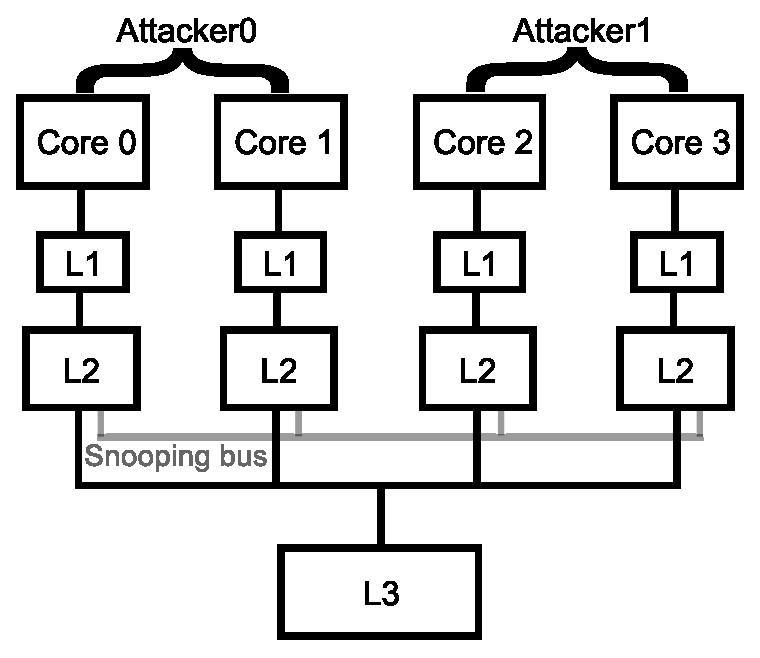
\includegraphics[width=2.3in]{figs/coherent_system.eps}
        \caption{Configuration for a covert channel attack.}
        \label{fig:coherent_system}
    \end{center}
\end{figure}

Attacker0 has two threads, each running on a different core. Both threads run a 
$\mathtt{for }$ loop of 4000 iterations, and
write to a shared data in each iteration. Before each write is performed, one 
L2 cache has to forward the data
to the other L2 cache through the snooping coherence bus and invalidates its own copy, 
according to the cache coherence protocol.  As a result, there is a lot of 
coherence traffic between these two threads. Attacker0 runs this $\mathtt{for }$ loop 
repeatedly and
records the time to finish the $\mathtt{for }$ loop.% using a C++ timing functions.

Attacker1 owns the secret data ('01101100') and tries to communicate this 
secret to Attacker0. It checks each bit
in the secret data. If the bit is 0, it executes a $\mathtt{for }$ loop only with a 
single thread.
This does not produce coherence traffic. If the bit is 
1, Attacker1 spawns a new thread, which also runs a $\mathtt{for }$ loop that writes to 
the same data, hence producing a lot of coherence traffic. 

\begin{figure}
    \begin{center}
        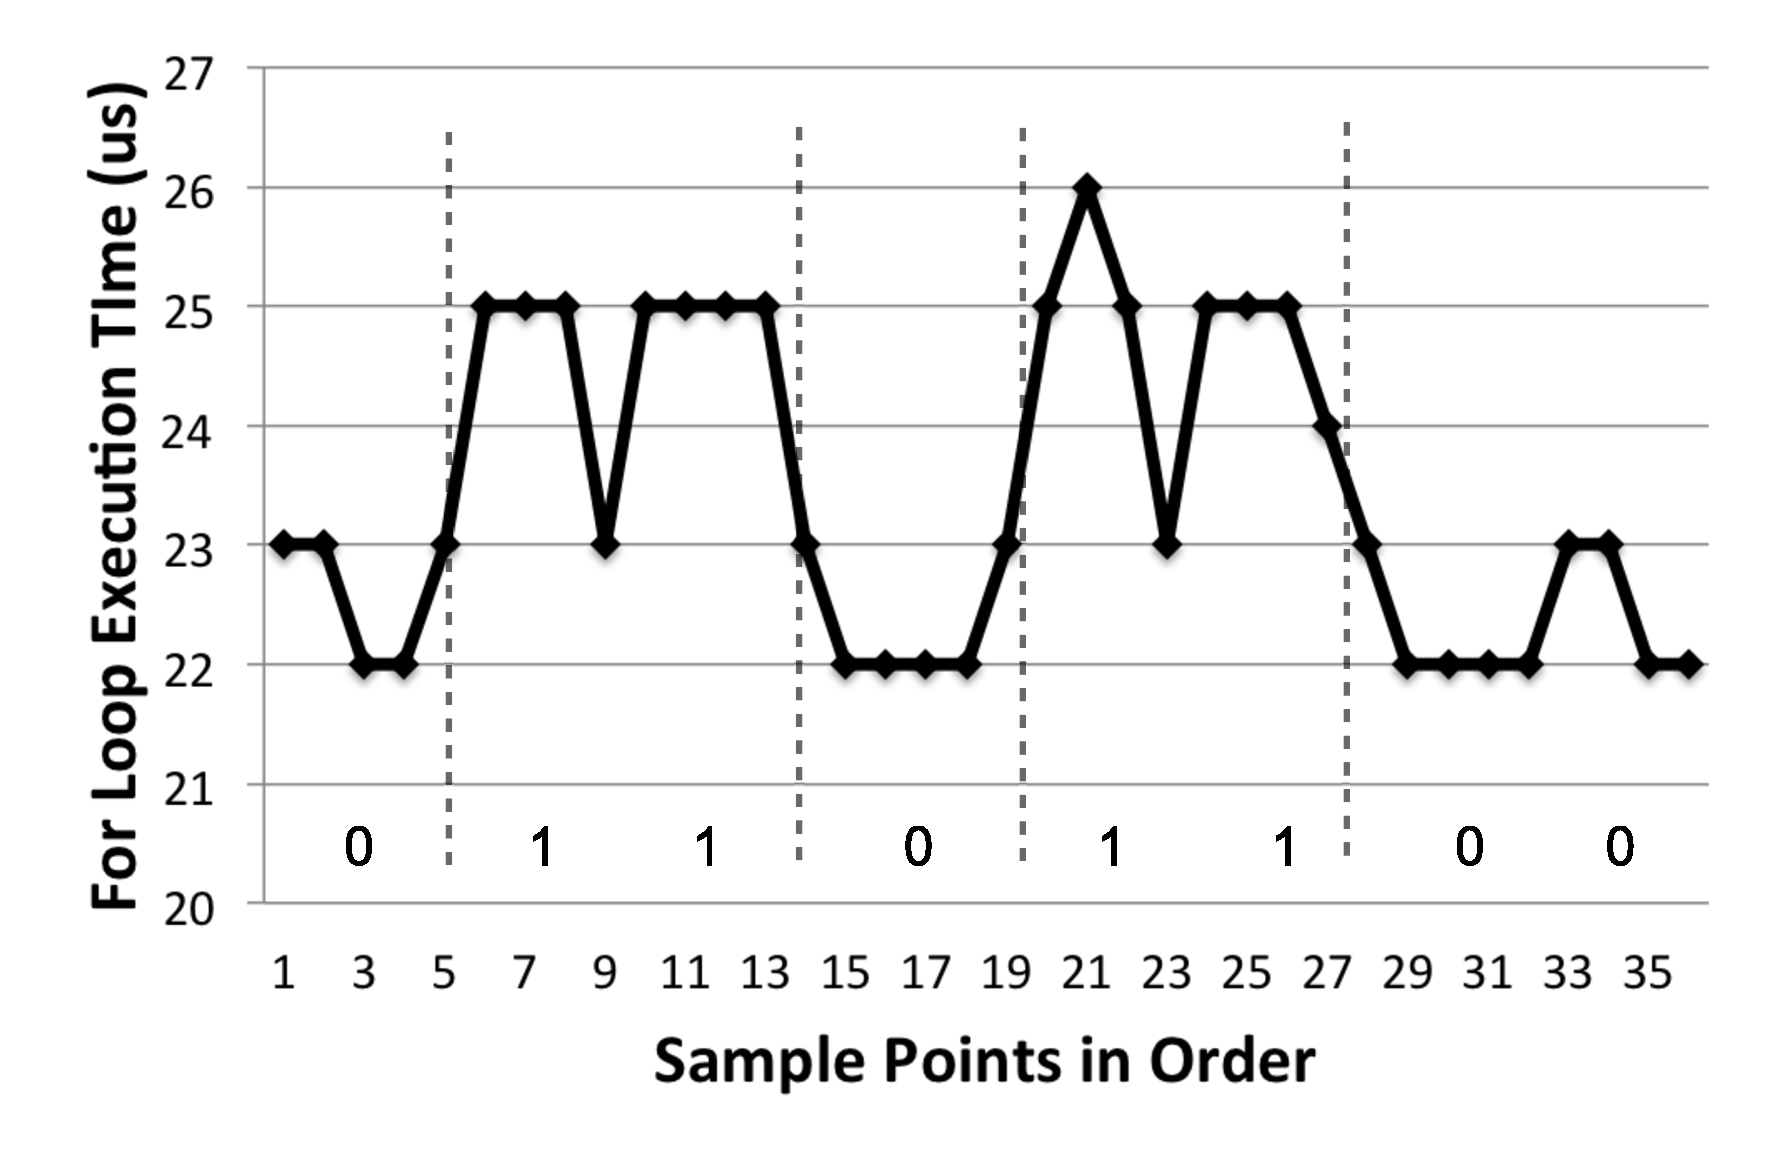
\includegraphics[width=2.79in]{figs/coherence_interference.eps}
        \caption{Attacker0's timing observation.}
        \label{fig:coherence_interference}
    \end{center}
\end{figure}

Note that in this example, we have all the aforementioned protection schemes 
implemented except for the snooping coherence bus.
Figure~\ref{fig:coherence_interference} shows the execution time of the $\mathtt{for }$ 
loop that Attacker0 observes. Each
sample point represents the time it takes to finish a 4000 iteration of the $\mathtt{for }$ 
loop. Based on the observation, Attacker0
can recover the secret successfully. The timing variation is caused by the 
interference on the snooping bus. If Attacker1
produces a lot of coherence traffic, Attacker0's coherence traffic gets delayed 
and thus finishes slower compared to
when Attacker1 does not produce coherence traffic. 

{\bf Bus Contention}
The protection for cache coherence mechanisms need to deal with two sources of
timing interference: bus contention and data array port contention.
To remove the interference on the snooping coherence bus, the bus
uses TDM. Each coherence request is tagged with a TCID of the core that
initiates the request so that it can only be send during that TC's bus turn.
Similarly, a coherence response is restricted to a particular bus turn.
Unlike requests, however, the responses are marked with the TCID of the
corresponding request, not the core's TCID.
This protection is similar to what we used for on-chip interconnect. 

{\bf Data Array Port Contention}
The second source of interference comes from a port contention for a cache
data array. As explained above, in the MOESI protocol, the cache that owns 
data may need to send data. However, reading data from a cache array for
a coherence request may interfere with a request from a processing pipeline.
We solve this contention problem by having the data served by the shared
cache or memory rather than reading a copy in a private cache if a
coherence request is from a timing compartment that is different from
the one that the private cache belongs to.
Because there can only be shared read-only data between timing compartments,
the shared cache or memory should always have an up-to-date copy.

%The second part deals
%with the shared data. Since the shared data is read-only, the cache miss does 
%not necessarily have to be served by
%the cache that has the Owned copy. Instead, the cache miss can always be served 
%by the next level of cache or memory.
%In our mechanism, when the cache receives a snooping request, it will first 
%check if the TCID of the request matches its
%own TCID. If the TCIDs mismatch, then the cache ignores the snooping request 
%even if it has the data, effectively acting
%as if the data does not exist. Then the cache miss will be served by the next 
%level of cache. A tricky thing here is
%coordinating the operations of multiple level of caches. In some protocols (e.g 
%MOESI), the cache that has the Owned copy
%is responsible for responding to the snooping request, so the next level of 
%cache does not respond. In this case, the
%cache needs to notify the next level of cache to respond to the snooping 
%request. The notification message should
%have a TCID that's the same with the requses so that it does not interfere with 
%its own snooping requests on the snooping bus. With our design, the cache that 
%sends a snooping request does not know the data exists on the other cache, 
%while
%the timing of the other cache's own operations is not affected.
 
\subsection{Private Per-Core Resources}

The resources that are dedicated to each core such as private caches,
TLBs, and branch predictors, are only used by one timing compartment at a time.
However, multiple timing compartments can use these resources through 
time-sharing. Therefore, there exist state-based timing channels if the state 
is
kept across context switches. For example, the number of cache blocks that
are evicted by one compartment may affect the number of cache hits for
another compartment in the following time slice.
We eliminate these timing channels by flushing the per-core resource state on a 
context switch that moves to a different timing compartment.
Therefore, the hardware needs to support the flushing operation.

%This is handled in software by the timing compartment manager and
%does not 
%(see 
%Section~\ref{sec:integration_tcm}).

%\subsection{Other System Resources}

%Talk about DMA, I/O, etc. Managed by SW.
